\documentclass[10pt,a4paper]{article}

\usepackage[margin=0.92in]{geometry}
\usepackage{amsmath,amssymb}
\usepackage{graphicx}
\usepackage{booktabs}
\usepackage{caption}
\usepackage[hidelinks]{hyperref}
\usepackage{microtype}

\graphicspath{{../web/figures/}}
\captionsetup{font=small,labelfont=bf}
\setlength{\parskip}{0.25em}

\title{\textbf{Mechanism Design: Is It Ever Worth Lying in an Auction?}}
\author{
Sreenitya Thatikunta (B23CS1072) \\
Prajna Agrawal (B23CS1054) \\
Arpita Deshmukh (B23CM1007)
}
\date{November 2026}

\begin{document}
\maketitle

\section{What we are asking}

An auction is just a set of rules. Everyone writes down a number, and the rules decide who
wins and how much they pay. The question we care about is whether those rules make honesty
a good idea.

A rule is called \emph{strategyproof} (or truthful) if telling the truth is your best move
no matter what the other bidders do. That sounds like a big promise, but it is narrower
than it looks. It does not say honesty will make you a lot of money, and it does not say
honesty is your \emph{only} good move. It only says nothing else does better.

That last point matters more than we expected when we started, so we want to flag it
early. There is a difference between honesty beating every other bid (called
\emph{strictly} dominant) and honesty never losing to another bid but often tying with it
(\emph{weakly} dominant). The second-price auction is only the second kind, and we report
the ties instead of hiding them. Section~\ref{sec:second} goes into this.

\begin{table}[h]
\centering
\small
\begin{tabular}{llll}
\toprule
& \textbf{Auction} & \textbf{Is honesty the best move?} & \textbf{What honesty pays you} \\
\midrule
Part 1 & Second-price, 1--2 rivals & Yes, weakly & Your full profit, $v - m$ \\
Part 2 & First-price, $n = 2, 3, 4$ & \textbf{No}; the best bid is $k = (n-1)/n$ & Exactly $0$ \\
Part 3 & VCG cheapest path & Yes & What you add to the network \\
\bottomrule
\end{tabular}
\caption{Our three results in one place.}
\end{table}

One piece of vocabulary before we start. Your \emph{value} $v$ is what the item is worth to
you, and only you know it. Your \emph{utility} is your profit: $v - p$ if you win and pay
$p$, and $0$ if you lose.

\section{The second-price auction}
\label{sec:second}

\subsection{How it works}

Bidder 1 (us, in this setup) has a value $v$ fixed at $0.2$, $0.5$ or $0.8$, and bids some
$b$ from the list $0.00, 0.01, \dots, 1.00$. There are one or two rivals. Each rival draws
its own value from $U[0,1]$, meaning any number between $0$ and $1$ is equally likely, and
then bids in one of three ways: honestly, at half its value, or by picking a fresh $U[0,1]$
number and ignoring its value completely.

The highest bid wins, but the winner pays the \emph{second} highest bid. So if we win, we
pay $m$, the biggest rival bid, and our profit is $v - m$. If we lose we get $0$. Three
values, three rival behaviours and two rival counts gives us 18 cases to look at.

\subsection{Why honesty wins here}

Look closely at that profit, $v - m$. Our own bid $b$ is not in it. This is the whole
reason the auction works: our bid decides \emph{whether} we win, but it never decides
\emph{what we pay}. So changing our bid cannot make any auction cheaper or more expensive.
All it can do is move the line between the auctions we win and the ones we lose. So ask
which auctions get moved:

\begin{itemize}
\itemsep0.15em
\item \textbf{Bid above your value.} You now also win the auctions where $m$ landed between
$v$ and $b$. In all of those you pay more than the item is worth to you, so your profit is
negative. You have bought yourself a pile of losses and gained nothing.
\item \textbf{Bid below your value.} You now lose the auctions where $m$ landed between $b$
and $v$. In all of those you would have paid less than the item was worth, so you have
thrown away profit.
\end{itemize}

\noindent
Both directions are bad, and $b = v$ is the line between them. We like this argument
because it works auction by auction and needs no probability at all.

The averages agree. If there are $k$ rivals and each one bids uniformly on $[0, s]$, then
the highest rival bid is below $m$ with probability $(m/s)^k$. Writing $t = \min(b, s)$,
\begin{equation}
\mathbb{E}[u(b)] = \int_0^{t} (v - m)\, d\!\left[(m/s)^k\right]
= \left(\frac{t}{s}\right)^{\!k}\!\left(v - \frac{kt}{k+1}\right),
\qquad
\frac{d\mathbb{E}}{db} = (v - b) f(b).
\label{eq:sp}
\end{equation}
The $f(b)$ is a probability density, so it is never negative. That means the sign of the
derivative is just the sign of $(v - b)$: positive when $b < v$ and negative when $b > v$.
The curve climbs up to $b = v$ and comes back down after it. The $t = \min(b, s)$ part is
there because if a rival can never bid above $s$, then bidding above $s$ gains us nothing,
since we are already winning everything.

\begin{figure}[t]
\centering
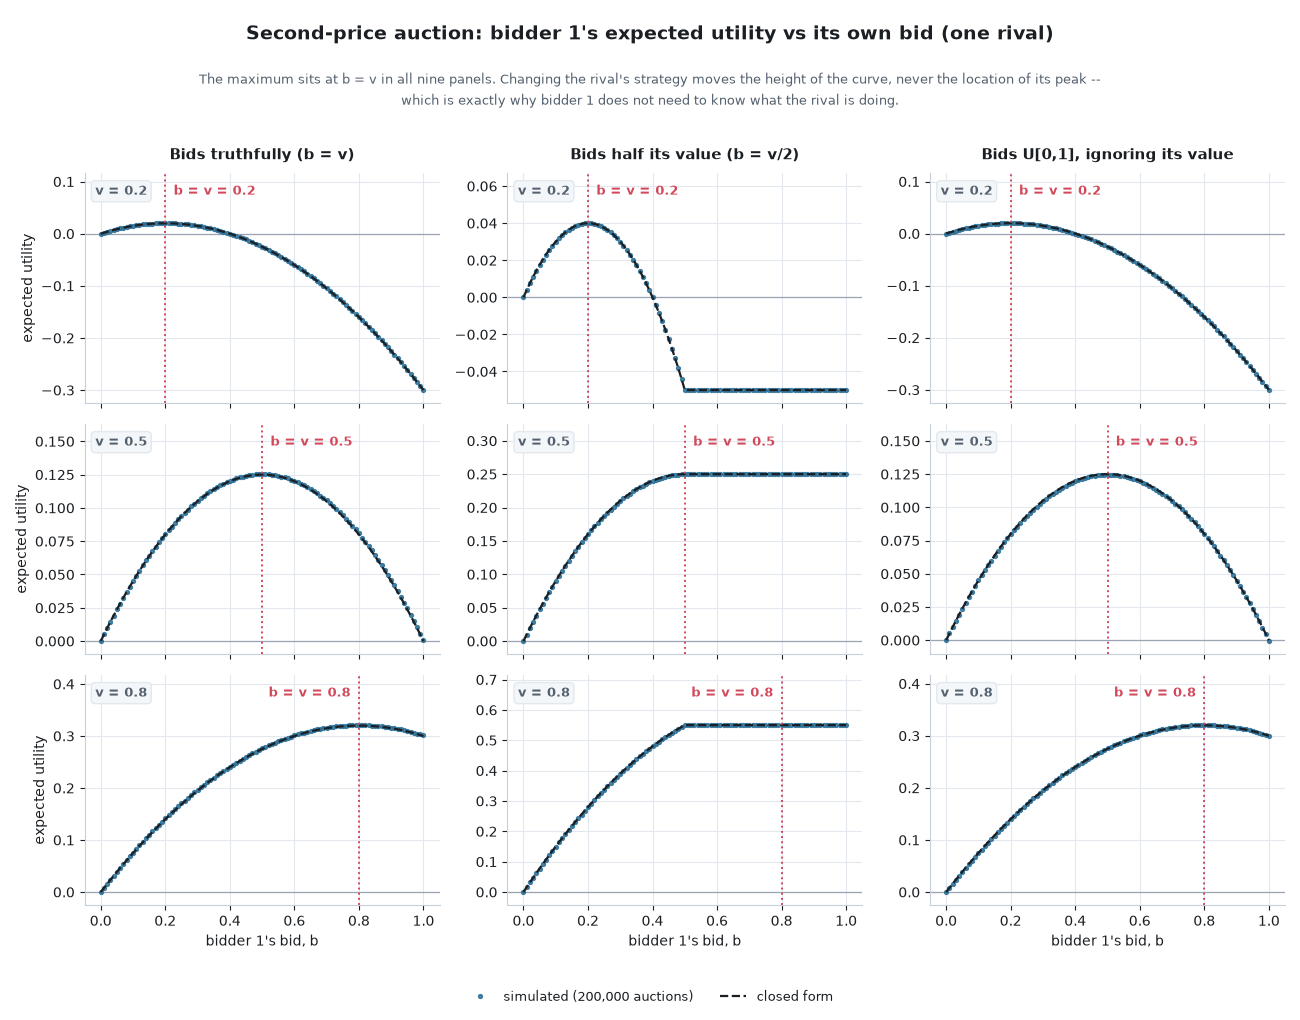
\includegraphics[width=0.55\textwidth]{part1a_second_price_1rival.png}
\caption{Expected profit for every bid, against one rival. The simulation and the formula
from Equation~\eqref{eq:sp} are drawn on top of each other. The curves change shape across
the nine panels, but the peak does not move.}
\label{fig:sp9}
\end{figure}

\subsection{What the plots told us}

Figure~\ref{fig:sp9} is useful because of what the nine panels share, not what makes them
different. The peak is at $b = v$ in every single one. That means we can pick our bid
without knowing which strategy the rival is using, which is what dominance is good for in
practice. Two other things stood out:

\begin{itemize}
\itemsep0.15em
\item \textbf{The first and third columns are identical.} A rival that bids its value draws
that value from $U[0,1]$, so its bid is spread uniformly over $[0,1]$. A rival that ignores
its value and picks a fresh $U[0,1]$ bid is spread the same way. From our side of the table
these two rivals look exactly the same, so no simulation could ever tell them apart.
\item \textbf{The middle column flattens out.} A rival bidding half its value never goes
above $0.5$, so once we bid $0.5$ we are already winning every auction. For $v = 0.8$ the
best answer is not a single point but the whole flat stretch from $0.5$ to $1.0$, which
happens to contain $b = v$. That is 51 bids tied for best.
\end{itemize}

Adding a second rival pushes all the curves down, because we win less often and pay more
when we do win. The peak stays at $b = v$ though. More competition changes how much we
make, not what we should do.

\subsection{Honesty ties a lot}

Against one \emph{fixed} rival bid, honesty is the best move but usually not the only one.
Say the rival bids $0.1$ and our value is $0.5$. Then bidding $0.2$, $0.5$ or $1.0$ all win
and all pay $0.1$. Three different bids, same result. Across our 18 fixed-bid cases,
somewhere between 41 and 91 of the 101 possible bids tied for best. We report the whole set
of best bids and how big it is, because picking one of them and calling it the answer would
make honesty look stronger than it really is.

There is one case where honesty is strictly best: $v = 0.8$ against a rival bidding $0.9$.
Bidding honestly loses, which pays $0$. Any bid that wins pays $0.9$ for something worth
$0.8$, losing $0.1$. Here losing is the best outcome available, and honesty is the only way
to get it.

\begin{figure}[h]
\centering
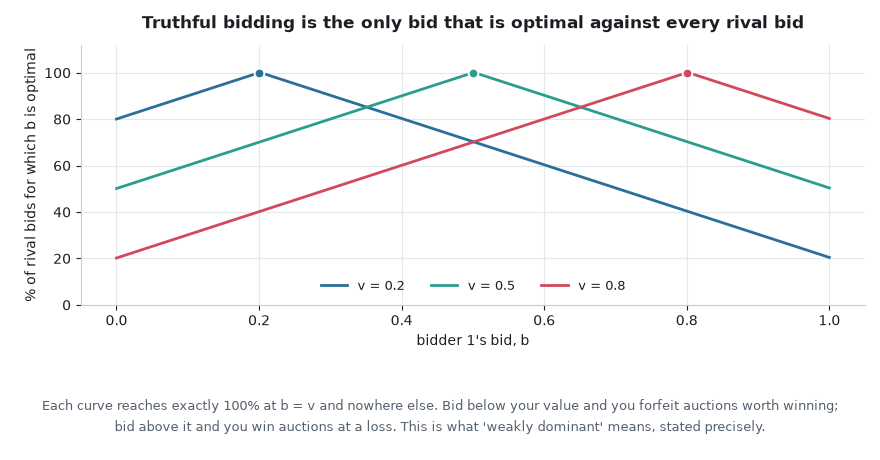
\includegraphics[width=0.58\textwidth]{part1_dominance_profile.png}
\caption{For each of our bids, the share of rival bids in $[0,1]$ that it is the best reply
to. Only $b = v$ reaches $100\%$.}
\label{fig:dom}
\end{figure}

Since no single rival bid singles out honesty, we tested it differently. We swept the
rival's bid across the whole range $[0,1]$ in 201 steps, and for each of our own bids we
counted how often it was the best reply (Figure~\ref{fig:dom}). Only $b = v$ wins every
time. Any bid below $v$ gives up auctions when the rival bids between $b$ and $v$, and any
bid above $v$ wins at a loss when the rival bids between $v$ and $b$. That is exactly what
weak dominance means, and checking only three fixed rival bids would not have shown it.

\section{The first-price auction}

\subsection{Being honest pays nothing}

Now all $n$ bidders draw values from $U[0,1]$, and the winner pays its own bid. Bidders
$2$ to $n$ play the known equilibrium strategy $b = c\,v$, where $c = (n-1)/n$. We bid
$k v$ instead, trying $k$ from $0.1$ up to $2.0$. Here $k = 1$ means bidding honestly. If
we win, our profit is
\begin{equation}
v - k v = v(1 - k),
\end{equation}
and at $k = 1$ that is zero. Every time. In a first-price auction, bidding what the item is
worth to you means handing over your entire profit whenever you win. The answer is not
small or noisy, it is exactly $0$.

What surprised us is how quiet this failure is. Bidding honestly still wins between $44\%$
and $75\%$ of the auctions, depending on $n$. You are not losing, you are winning
constantly and getting nothing for it. This is the sharpest contrast with
Section~\ref{sec:second}, and the reason is simple: here your bid \emph{is} your price.

\subsection{So how much should you shave off?}

You have to bid below your value, but not too far below. Shave too little and each win is
barely worth anything. Shave too much and you stop winning. The best answer is somewhere in
between. Let $M$ be the highest rival value. We win when $k v > c M$, so our chance of
winning is $\min(1, kv/c)^{n-1}$, and
\begin{equation}
\mathbb{E}[U(k)] = (1-k)\int_0^1 v \min\!\left(1, \tfrac{kv}{c}\right)^{\!n-1} dv
= \frac{(1-k)(k/c)^{n-1}}{n+1} \quad (k \le c).
\end{equation}
Maximising $(1-k)k^{n-1}$ gives $k = (n-1)/n$, and the profit there works out to the neat
$1/\big(n(n+1)\big)$. Notice that $k$ gets bigger as $n$ does. With two bidders you bid
half your value; with four you bid three quarters. The more competition there is, the less
you can afford to shave.

\begin{figure}[h]
\centering
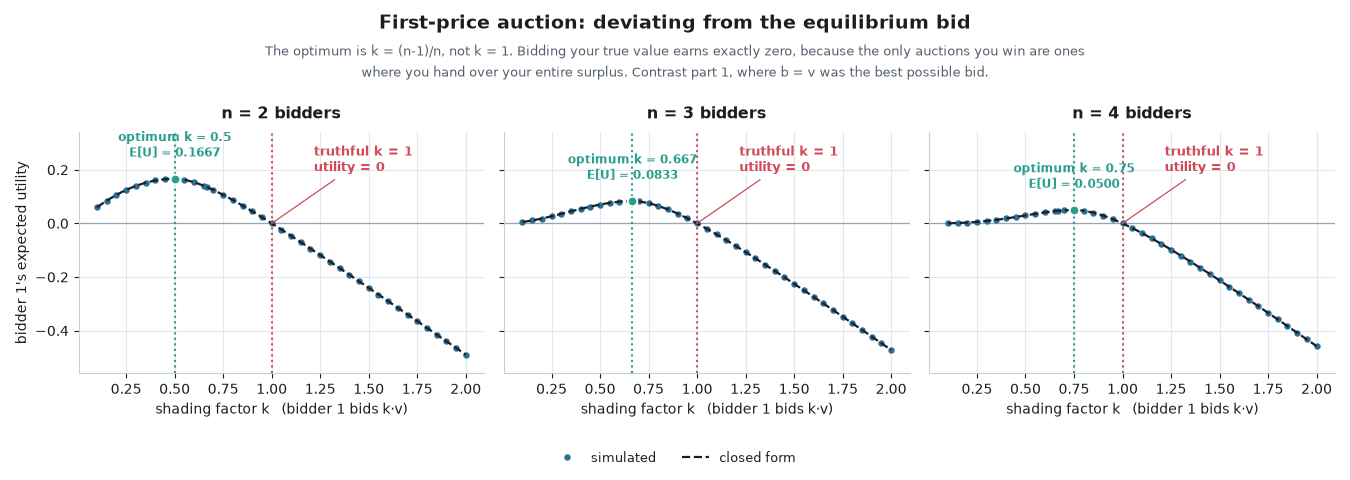
\includegraphics[width=0.88\textwidth]{part2_first_price_shading.png}
\caption{Expected profit against the shading factor $k$. The peak is at $k = (n-1)/n$,
honest bidding at $k = 1$ earns zero, and anything past $k = 1$ loses money.}
\end{figure}

\begin{table}[h]
\centering
\small
\begin{tabular}{cccccc}
\toprule
$n$ & Equilibrium $k$ & Our simulated best $k$ & Exact $1/(n(n+1))$ & Simulated & Profit at $k=1$ \\
\midrule
2 & 0.5000 & 0.5000 & 0.166667 & 0.166455 & 0 \\
3 & 0.6667 & 0.6667 & 0.083333 & 0.083307 & 0 \\
4 & 0.7500 & 0.7500 & 0.050000 & 0.049867 & 0 \\
\bottomrule
\end{tabular}
\caption{Our simulated best bid lands on the exact theory for every $n$.}
\end{table}

One thing tripped us up here, and it is worth writing down because it looks like a wrong
answer rather than a mistake. The number $2/3$ is not on a grid of $0.05$ steps. We had
been testing $k$ on such a grid, so for $n = 3$ our best $k$ came out as $0.65$. It looked
like the simulation had almost matched the theory and just missed, when really the correct
answer was never on the list of things we tried. We fixed it by adding the exact values
$(n-1)/n$ into the grid. The lesson we took from it is that a problem with your grid can
look identical to a real finding unless you already know the answer.

\subsection{What charging the winner's own bid costs}

We were also asked how often the winner could have bid less and still won. The answer is
$100.00\%$ of the time, and on its own that number tells you almost nothing. Bids come from
continuous distributions, so the winner almost always beats the runner-up by some small
amount, which means it almost always could have bid a little less. It is $100\%$ for every
first-price auction, whatever $n$ is. What actually tells you something is \emph{how much}
they overpaid.

\begin{table}[h]
\centering
\small
\begin{tabular}{cccc}
\toprule
$n$ & Could have paid less & Average overpayment & As \% of the winning bid \\
\midrule
2 & 100.00\% & 0.1664 & 49.9\% \\
3 & 100.00\% & 0.1665 & 33.3\% \\
4 & 100.00\% & 0.1502 & 25.0\% \\
\bottomrule
\end{tabular}
\caption{Winners pay a quarter to a half more than they needed to. In a second-price
auction this is always zero.}
\end{table}

In a second-price auction the winner pays the runner-up's bid exactly, so there is no gap at
all. That comparison is the real argument for charging the second price. Shading away from
equilibrium also messes up who wins: because we are bidding on a different scale from
everyone else, the winner is sometimes not the bidder who wanted the item most. So
deviating costs efficiency as well as profit.

\section{VCG for buying the cheapest path}

\subsection{The setup and the payment rule}

This last one is a different kind of problem. We have a network with nodes $A$ to $F$. Each
\emph{edge} is owned by someone who knows privately what it costs them, and we want to buy
a path from $A$ to $F$. Since we are buying rather than selling, the efficient choice is
the cheapest reported path. VCG pays an edge $e$ on the chosen path $P$ the amount
\begin{equation}
p_e = L(G \setminus e) - \big(L(P) - c_e\big),
\label{eq:vcg}
\end{equation}
which is the cost of the best path we could have used if $e$ did not exist, minus what the
rest of the chosen path costs us.

\begin{figure}[h]
\centering
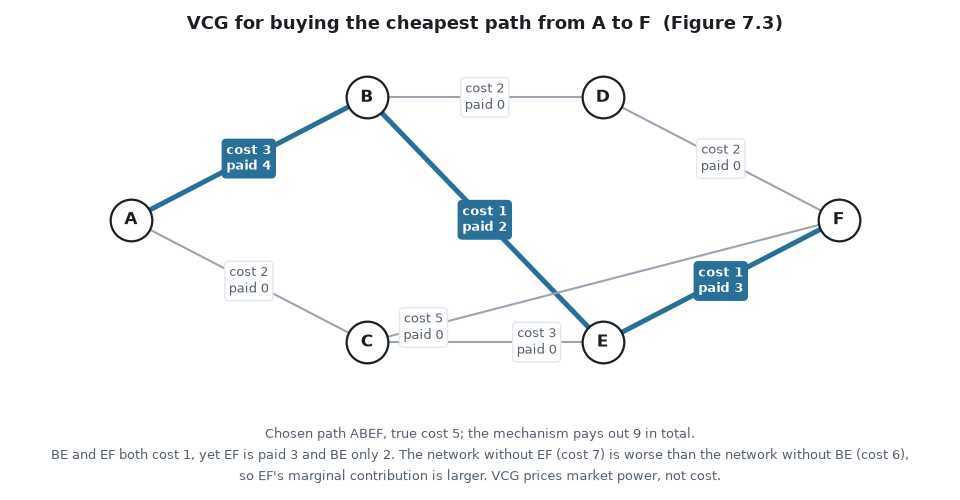
\includegraphics[width=0.56\textwidth]{part3_vcg_network.png}
\caption{The network from Figure 7.3 of Shoham and Leyton-Brown. The cheapest path is
$ABEF$ at $5$. $ACEF$ costs $6$, and $ABDF$ and $ACF$ both cost $7$.}
\label{fig:net}
\end{figure}

Here is why nobody can gain by lying. The piece $L(P) - c_e$ is just the cost of the
\emph{other} edges on the path. So both halves of Equation~\eqref{eq:vcg} are built only
out of what everybody else reported, and an edge's own report is not in its payment at all.
Lying cannot change what you get paid. The only thing it can change is whether you are on
the path, and since being on the path pays you something and being off it pays zero, the
only thing lying can do is accidentally price you off a path you wanted. Edges that are not
on the path get $0$, and that falls out of the formula rather than being a special rule: if
removing an edge does not change the chosen path, the two terms are equal and cancel.

\subsection{What we got}

\begin{table}[h]
\centering
\small
\begin{tabular}{lccccc}
\toprule
Edge & Cost & On the path & Best path without it & Paid & Profit \\
\midrule
$AB$ & 3 & yes & $ACEF$ (6) & \textbf{4} & 1 \\
$BE$ & 1 & yes & $ACEF$ (6) & \textbf{2} & 1 \\
$EF$ & 1 & yes & $ABDF$ (7) & \textbf{3} & 2 \\
$AC, BD, CE, CF, DF$ & 2 to 5 & no & $ABEF$ (5) & 0 & 0 \\
\bottomrule
\end{tabular}
\caption{The VCG payments, which match the textbook exactly.}
\end{table}

The interesting bit is that $BE$ and $EF$ both cost $1$, but $EF$ gets paid $3$ while $BE$
only gets $2$. VCG does not pay you for your cost, it pays you for how much you help. Take
$BE$ away and the best path left is $ACEF$ at $6$, so we are worse off by $1$. Take $EF$
away and the best path left is $ABDF$ at $7$, so we are worse off by $2$. Losing $EF$ hurts
twice as much, so $EF$ gets twice as much. Same cost, different amount of leverage.

We also checked the lying directly. For each edge we kept its true cost fixed and swept the
cost it \emph{reported} from $0$ to $10$ in steps of $0.5$. For $AB$, which is on the path
and truly costs $3$, the payment stayed at $4$ no matter what it reported, which is just
what the cancellation above predicts. Reporting less changed nothing, and reporting more
than about $4$ pushed it off the path and dropped its profit from $1$ to $0$. For $AC$,
which is off the path and truly costs $2$, reporting under $1$ did get it onto the path,
but then it was paid only $1$ for something that cost it $2$, so it lost $1$. The only way
to win was to win at a loss, which is the same trap as overbidding in
Section~\ref{sec:second}. Our tests run this sweep on all eight edges, not just these two,
and honesty is among the best options every time.

VCG is not free, though. It pays out $9$ in total for a path that really costs $5$, which is
$80\%$ more than the path is worth. That gap is what truthfulness costs the buyer, and it
is why VCG does not balance its budget when you use it to buy things.

\section{How we checked our work}

If you only ever check a simulation against another simulation, you can be confidently
wrong. We also did not want to use snapshot tests, where you save the output of a run that
looked right and check that later runs still match it, because that only proves the code
has not changed its mind, not that it was ever correct. All three of these auctions can be
solved exactly on paper, so we worked out a formula for every quantity we simulated and
made the tests compare the simulation to the formula. The plots show both lines together.
Across all 18 second-price cases the worst gap was $0.0016$.

Those formulas assume each rival's bid is spread uniformly over $[0, s]$. Everything
analytic in this report leans on that, so we tested it too, by comparing each strategy's
actual distribution of bids against the one we claimed it had, instead of just assuming it.
Four other choices are worth mentioning:

\begin{itemize}
\itemsep0.1em
\item \textbf{The same random draws for every bid.} We generate one batch of rival draws
per case and reuse it across the whole bid grid. Each average is still correct, but the
differences between neighbouring bids get much less noisy, so the shape of the curve, which
is what we actually want from the plot, comes out far cleaner for the same amount of work.
\item \textbf{Reporting all the best bids, not one.} Where lots of bids tie, we list them
all. Picking one would make weak dominance look like strict dominance.
\item \textbf{Breaking path ties on purpose.} The network has real ties, since $ABDF$ and
$ACF$ both cost $7$. Our Dijkstra breaks them by taking the alphabetically smallest
sequence of nodes. If we had left it to whatever order the heap happened to produce, our
test would have passed for the wrong reason. Doing it explicitly also meant our separate
JavaScript version matched the Python at all 42 points of the misreporting sweep, which is
better evidence than either one passing its own tests.
\item \textbf{Making it reproducible.} There is one master seed, and each part gets its own
stream from it, so any part can be rerun on its own and give the same numbers. Our CI reruns
the whole thing and fails if any committed number changed. We left the figures out of that
check on purpose: Matplotlib draws text using whatever fonts the machine has, so the same
plot built on macOS and on Linux differs byte for byte while looking identical, and checking
those bytes would be testing the fonts rather than our code.
\end{itemize}

\section{What we conclude}

One idea ties all three results together: \textbf{an auction is safe to be honest in exactly
when your own report cannot change your own price.} The second-price auction manages this by
charging you the runner-up's bid. VCG manages it by building your payment only out of what
other people reported. The first-price auction breaks it in the most direct way possible,
since your bid is your price, and that one fact is why honesty there is worth nothing. No
amount of good intentions on a bidder's part can fix it, because the problem is in the rules
and not in the people following them.

Two things we want to be careful about. First, the dominance in Section~\ref{sec:second} is
weak and not strict. Honesty never loses, but it ties with other bids very often, and we
reported how often rather than glossing over it. Second, strategyproofness is something you
pay for. VCG's $80\%$ premium on this network is the price of getting everyone to tell the
truth.

\vspace{1em}
\noindent\textbf{Reference.} Y. Shoham and K. Leyton-Brown, \emph{Multiagent Systems:
Algorithmic, Game-Theoretic, and Logical Foundations}, Cambridge University Press.
Chapter 7, with Figure 7.3 and the worked VCG example in \S4.2.

\end{document}
